\section{The whole macromolecule}

To regenerate the whole human \ttt{metHgb} macromolecule, $Chimera$ \ttt{operate} and assessment - refinement -assessment protocols will be used. Starting from the unit cell, $Chimera$ \ttt{operate} protocol allows to generate the whole molecule by symmetry. As in the previous step, validation programs drive to selection of the best $model$ of the whole molecule after one or several rounds of assessment - refinement -assessment. A final validation step will be accomplish with $Chimera$ \ttt{operate} protocol to assess volume density occupancy.

\begin{itemize}

 \item Protocol \scommand{chimera operate} to generate the whole molecule of human \ttt{Hgb}:\\
 
 Following previous instructions, open $Chimera$ \ttt{operate} protocol (\ffigure{fig:chimera_operate_protocol} (1)), load 
 the selected atomic structure $model$ of \ttt{metHgb} unit cell (2), and execute the protocol (3). $Chimera$ graphics interface will show you the $model$ of \ttt{metHgb} unit cell. Considering the C2 symmetry of the whole molecule, write in $Chimera$ command line to re-generate the whole molecule:\\
 
 \ttt{sym \#2 group C2}\\
 
 A symmetric image of the input $model$ (\ffigure{fig:chimera_operate_sym}; \#2) will be generated (\#3). $Model$ \#1 is the initial extracted unit cell volume associated to \ttt{metHgb} unit cell $model$ loaded. By selecting $models$ \#2 and \#3, and pressing \ttt{Copy/Combine} in the right side of \ttt{Model Panel}, a new $model$ \#4 is generated. This new $model$ contains the four subunits that integrate the two symmetric unit cells. The whole molecule $model$ can be saved by writing in $Chimera$ command line:\\
 
 \ttt{scipionwrite model \#4 refmodel \#1 saverefmodel 0}\\
 
 \begin{figure}[H]
    \centering 
    \captionsetup{width=.7\linewidth} 
    \includegraphics[width=0.90\textwidth]{Images/Fig41}
    \caption{$Model$ generated for the whole human \ttt{metHgb}.}
    \label{fig:chimera_operate_sym}
   \end{figure}
 
 \item Validation protocols to select the best $model$ of the whole human \ttt{Hgb}:\\
 
 $EMRinger$ and $MolProbity$ statistics have to be computed for the new $model$ of the whole human \ttt{metHgb} obtained by using $Chimera$ \ttt{operate} protocol (see results \ttable{table:refmac_question_12} in Appendix \ref{app:solutions}; \textbf{Question 12}). Because of high values of \ccmask and $EMRinger$ \ttt{score}, as well as acceptable $MolProbity$ statistics, $model$ generated by $Chimera$ \ttt{operate} protocol is selected as $model$ of the whole human \ttt{metHgb}. Additional refinement steps with $Phenix$ \ttt{real space refine} and $Refmac$ do not seem to improve the result significantly. In this case, RMSD value of the selected atomic structure $model$ regarding the published structure yields an intermediate value between the best and the worst one.\\
 
 \item Protocol \scommand{chimera operate} to assess volume density occupancy:\\
 
 As we have seen previously, open $Chimera$ \ttt{operate} protocol (\ffigure{fig:chimera_operate_protocol} (1)), load both the initial volume and the selected atomic structure $model$ of the whole human \ttt{metHgb} (2), and execute the protocol (3). \ffigure{fig:chimera_operate_vol} shows the initial volume \ttt{EMD-3488} (grey) and the selected $model$ that we have traced for human \ttt{metHgb} (pink):
 
 \begin{figure}[H]
    \centering 
    \captionsetup{width=.7\linewidth} 
    \includegraphics[width=0.90\textwidth]{Images/Fig42}
    \caption{Human \ttt{metHgb} $model$ opened by $Chimera$ \ttt{operate} protocol.}
    \label{fig:chimera_operate_vol}
   \end{figure}
 
 To check if the selected model of \ttt{metHgb} occupies most part of the starting volume, we have to compare by subtraction the $model$-derived volume and the starting volume \ttt{EMD-3488}. To perform this operation, follow the next two steps:\\
 
  \begin{itemize}
  
  \item To generate a volume from the $model$ at 3.307\AA\ resolution (resolution shown in $Phenix$-\ttt{$MolProbity$ viewer}; \ttt{Real space correlation}; \ttt{Atom Mask Radius}), write in $Chimera$ command line:\\
  
  \ttt{molmap \#2 3.307 modelId 3}\\
  
  Next \ffigure{fig:chimera_operate_vol_2} shows the volume (\iii{Chimera model} \#3) generated in $Chimera$ at 3.307\AA\ resolution, starting from the selected atomic structure of human \ttt{metHgb} (\iii{Chimera model} \#2). 
   
  \begin{figure}[H]
    \centering 
    \captionsetup{width=.7\linewidth} 
    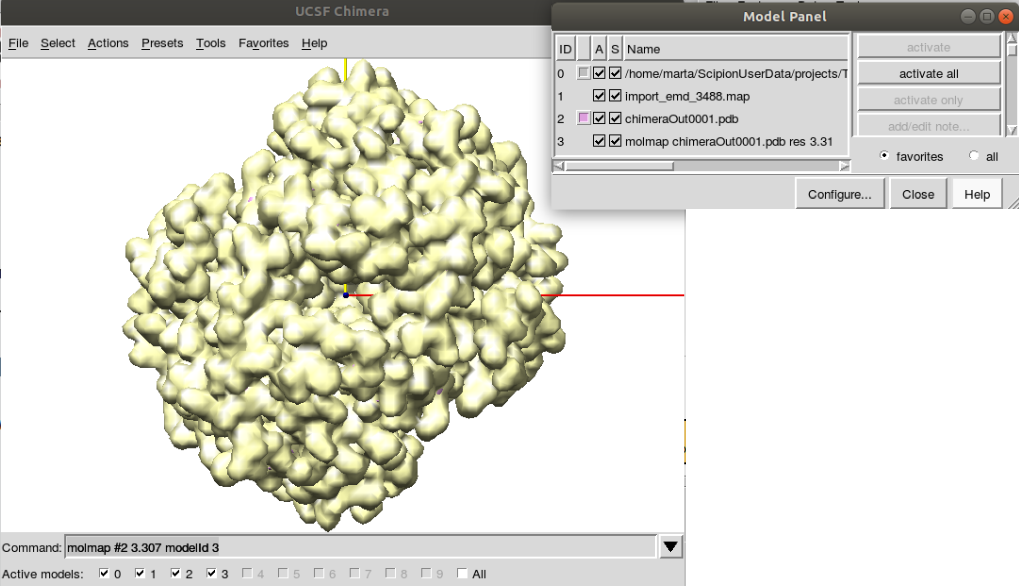
\includegraphics[width=0.90\textwidth]{Images/Fig43}
    \caption{Electron density volume generated from human \ttt{metHgb} $model$ in $Chimera$.}
    \label{fig:chimera_operate_vol_2}
   \end{figure}
  
  \item To subtract this new model from the starting whole volume \ttt{EMD-3488}, write in $Chimera$ command line:\\
  
  \ttt{vop subtract \#1 \#3 modelId \#4} \\
  
  Resulting volume from this subtraction operation appears in \ffigure{fig:chimera_operate_vol_3} (\iii{Chimera model} \#4). From this result, we can conclude that most part of the initial density map has been traced, and there are no significant additional densities others than the four monomers and the four prosthetic groups that we have considered so far.
  
  \begin{figure}[H]
    \centering 
    \captionsetup{width=.7\linewidth} 
    \includegraphics[width=0.90\textwidth]{Images/Fig44}
    \caption{Electron density difference between the starting volume \ttt{EMD-3488} and the volume generated from human \ttt{metHgb} $model$.}
    \label{fig:chimera_operate_vol_3}
   \end{figure}
  
  
  \end{itemize}
 
\end{itemize}
